\subsection{Análisis de datos}
El gran potencial analítico de la información generada por los puntos de control y el simulador
del proceso evolutivo, permiten la implementación diferentes tipos de análisis estadísticos y
geográficos. De forma básica se han implementado la cartografía del vector, la identificación de
focos y el análisis del ciclo de vida del vector.

\subsubsection{Cartografía del vector}
La cartografía del vector, es empleada para representar geográficamente la distribución espacial
del vector \citep{vgomesAegis2001}. Esta es obtenida a partir de los puntos de control establecidos
previamente, donde, cada uno se encuentra asociado a con nivel de criticidad
(\figref{fig:cap-5-cartografica-vector}).


\begin{figure}[!htpb]
\centering
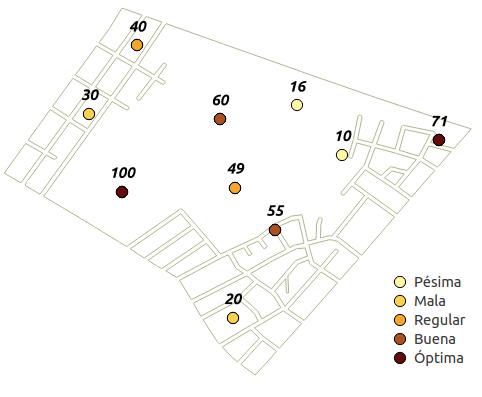
\includegraphics[width=0.6\textwidth]{capitulo-5/graphics/cartografia-vector.png}
\caption{\label{fig:cap-5-cartografica-vector}Ejemplo de cartografía del vector.}
\end{figure}

\subsubsection{Identificación de focos de infestación}
\label{sec:cap5-identificacion-focos}
El proceso de identificación de focos de infestación fue previamente presentado en la
\secref{sec:cap4-identificacion-focos}, es el encargado de transformar la información obtenida de
los puntos de control, distribuidos geográficamente, mediante métodos de interpolación, en mapas
donde se puede apreciar los niveles de riesgo correspondientes
(\figref{fig:cap-5-identificacon-focos}).

\begin{figure}[!htpb]
\centering
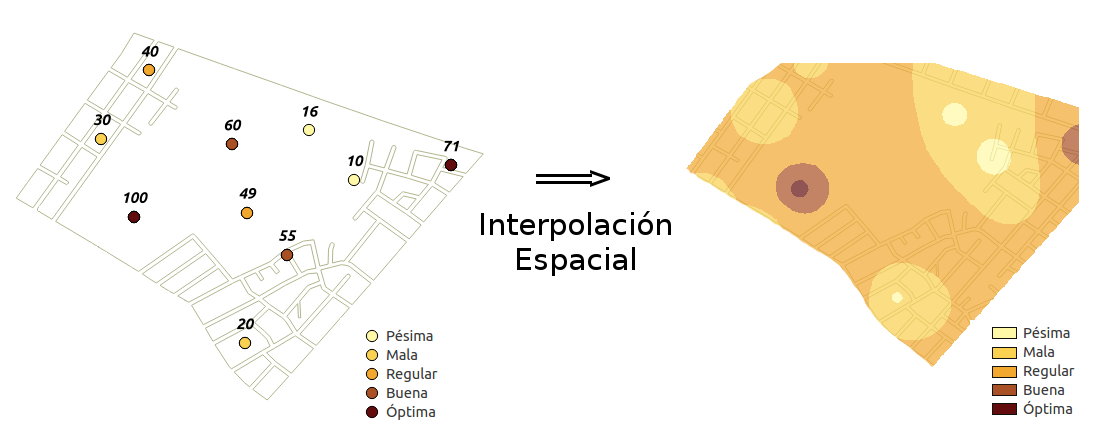
\includegraphics[width=1\textwidth]{capitulo-5/graphics/identificacion-focos.png}
\caption{\label{fig:cap-5-identificacon-focos}Ejemplo de transformación de puntos de control a mapas de interpolación.}
\end{figure}

La selección del método de interpolación se realizó teniendo en cuenta el factor humano en la
distribución de los puntos de control. En \cite{villatoro2007comparacion} se realiza una
comparación de los interpoladores IDW y Kriging, donde los autores señalan que el método Kriging
fue más preciso y eficiente que el IDW, aunque la diferencia entre ambos métodos no fue muy amplia.
Sin embargo, cuando el distanciamiento, es muy grande, los variogramas no son posibles de obtener,
entonces el Kriging deja de ser una opción y comparativamente el IDW se perfila como el mejor
\cite{villatoro2007comparacion}. El método seleccionado finalmente fue el IDW, debido que la
distribución del los puntos de control no será perfecta, inclusive, en algunas localidades la
distribución no será de forma uniforme.

\subsubsection{Análisis del ciclo de vida del vector}
El análisis del ciclo de vida del vector consiste en procesar la información generada durante el
proceso evolutivo para determinar :

\begin{itemize}
    \item \textit{Duración promedio del ciclo de vida}, determina la duración en días de cada etapa de desarrollo del vector, con esto podemos determinar que tan rápido puede desarrollarse al población.

    \item \textit{Tasa de mortalidad diaria} indica el porcentaje de reducción diario de la población.

    \item \textit{Duración del ciclo gonotrófico}, calcula la duración promedio, en días, del ciclo gonotrófico de las hembras adultas nulíparas y paridas.

    \item \textit{Rango de dispersión}, indica el radio promedio de vuelo, en metros, del adulto tomando como origen el lugar donde emergió.

\end{itemize}
